\documentclass[letter,11pt]{article}
%\documentclass[letter,twoside,11pt]{article}

\usepackage[spanish,es-nodecimaldot]{babel}
\usepackage[utf8]{inputenc}

\usepackage{lmodern}
\usepackage[T1]{fontenc}
\usepackage{textcomp}

\usepackage{graphicx}
\usepackage{pstricks}

\usepackage{anysize}
\marginsize{3cm}{2cm}{2cm}{3cm}

\usepackage{amsmath}
\usepackage{array}

\usepackage{fancyhdr}
\usepackage{lastpage}
\pagestyle{fancy}
\fancyhf{}
\fancyhead[LE,RO]{Laboratorio de Física Básica I}
\fancyfoot[CO,CE]{\thepage\ de \pageref{LastPage}}

\special{papersize=215.9mm,279.4mm}

\usepackage[
    pdfauthor={Carlos Eduardo Caballero Burgoa},%
    pdftitle={Laboratorio de Física Básica I},%
    pdfsubject={Medidas directas},%
    colorlinks,%
    citecolor=black,%
    filecolor=black,%
    linkcolor=black,%
    urlcolor=black,
    breaklinks]{hyperref}
\usepackage{breakurl}

\newcommand{\blankpage}{
    \newpage
    \thispagestyle{empty}
    \mbox{}
    \newpage
}

\renewcommand{\arraystretch}{1.2}

\begin{document}

\begin{titlepage}
\begin{center}
{\Large UNIVERSIDAD MAYOR DE SAN SIMÓN}\\
\vspace*{0.15cm}
{\large FACULTAD DE CIENCIAS Y TECNOLOGÍA}\\
\vspace*{0.10cm}
DEPARTAMENTO DE FÍSICA\\
\vspace*{3.0cm}
{\Large \textbf{LABORATORIO DE FÍSICA BÁSICA I}}\\
\vspace*{0.3cm}
{\Large \textbf{PRACTICA No. 1}}\\
\vspace*{3.5cm}
{\Large \textbf{MEDIDAS DIRECTAS}}\\
\end{center}

\vspace*{7.4cm}
\leftskip=7.95cm
\noindent
\textbf{Estudiante:}\\
Caballero Burgoa, Carlos Eduardo.\\
\newline
\textbf{Docente:}\\
Msc. Guzmán Saavedra, Rocio.\\
\newline
\textbf{Grupo:} N5.\\
\textbf{Fecha de realización:} 11 de Octubre del 2020.\\
\textbf{Fecha de entrega:} 13 de Octubre del 2020.\\

\end{titlepage}

\blankpage

\section{Objetivo}
Ejercitar la toma de datos, y la correcta presentación del resultado de la
medida.

\section{Marco teorico}
Los resultados de las medidas nunca se corresponden con los valores reales de
las magnitudes a medir, sino que, en mayor o menor extensión, son defectuosos,
es decir, están afectados de error. Las causas que motivan tales desviaciones
pueden ser debidas al observador, al aparato o incluso a las propias
características del proceso de medida.

Una medida directa es aquella, cuyo valor se consigue directamente por
comparación con la escala de un instrumento. Se pueden realizar en una sola
medición o en una serie de mediciones.

Si las fuentes de error son únicamente de carácter aleatorio, es decir, si
influyen unas veces por exceso y otras por defecto en el resultado de la medida,
puede demostrarse que el valor que más se aproxima al verdadero valor es
precisamente el valor medio. Ello es debido a que al promediar todos los
resultados, los errores por exceso tenderán a compensarse con los errores por
defecto y ello será tanto más cierto cuanto mayor sea el número de veces que se
repita la medición.

Si se realizan $n$ mediciones directas de una magnitud física, denotadas
por:

\begin{equation}
    \{x_1,x_2,x_3,\cdots,x_i,\cdots,x_n\}
\end{equation}

Para calcular el valor representativo de esta serie de mediciones, se toma la
media aritmética:

\begin{equation}
    \bar{x} = \frac{x_1+x_2+\cdots+x_n}{n} = \frac{1}{n}\sum_{i=1}^{n} x_i
\end{equation}

Para determinar el error en la medición, se hace uso de la desviación estándar,
que es una medida de dispersión usada en estadística que nos dice cuánto tienden
a alejarse los valores concretos del promedio en una distribución.

La desviación estándar ($\sigma$) es la raíz cuadrada de la varianza ($s^2$) de
la distribución de probabilidad discreta, y puede calcularse con la siguiente
formula:

\begin{equation}
    \sigma = \sqrt{s^2}
\end{equation}

Donde:

\begin{equation}
    s^2 = \frac{1}{n}\sum_{i=1}^{n} (x_i-\bar{x})^2
\end{equation}

Aunque esta fórmula es correcta, en la práctica interesa el realizar inferencias
poblacionales, por lo que en el denominador en vez de $n$, se usa $n-1$ según la
corrección de \emph{Bessel}.

\begin{equation}
    \sigma_{n-1} = \sqrt{\frac{\sum_{i=1}^{n} (x_i-\bar{x})^2}{(n-1)}}
\end{equation}

El error de la medida, es igual a la desviación estándar dividida por la raíz
cuadrada del número de mediciones.

\begin{equation}
    \sigma_x = \frac{\sigma_{n-1}}{\sqrt{n}}
             = \sqrt{\frac{\sum_{i=1}^{n} (x_i-\bar{x})^2}{n(n-1)}}
\end{equation}

Se define a $[(\bar{x}-\sigma_x), (\bar{x}+\sigma_x)]$ como el intervalo de
confianza en el que el valor verdadero de la medición puede encontrarse según un
porcentaje de confianza definido por el modelo de distribución de probabilidad.

Para el calculo del error $e_x$ de una serie de mediciones, es recomendable
colocar el mayor valor entre el error obtenido anteriormente $\sigma_x$ y la
precisión del instrumento de medida ($P$):

\begin{equation}
    e_x = \begin{cases}
        \sigma_x, & \mbox{si }\sigma_x > P \\
        P,        & \mbox{si }\sigma_x < P
    \end{cases}
\end{equation}

El error de la medición tambien debe representarse en su forma porcentual con la
siguiente formula:

\begin{equation}
    E\% = \frac{e_x}{\bar{x}}\cdot100
\end{equation}

Finalmente el resultado de las mediciones será:

\begin{equation}
    x = (\bar{x}\pm e_x)[u], E\%
\end{equation}

\section{Materiales}
\begin{itemize}
\item Distanciómetro.
\item Sonómetro.
\item Acelerómetro.
\item Luxómetro.
\end{itemize}

\section{Procedimiento}
A continuación se describen los procedimientos experimentales de medición que se
llevarán a cabo.

\subsection{Medición de distancia}
\begin{enumerate}
\item Armar un tripode para establecer una posición fija para la medición.
\item Medir la altura
\end{enumerate}

\subsection{Medición de la intensidad del sonido}
\begin{enumerate}
\item 
\end{enumerate}

\subsection{Medición de la gravedad}
\begin{enumerate}
\item 
\end{enumerate}

\subsection{Medición de la intensidad de la luz}
\begin{enumerate}
\item Armar un tripode para establecer una posicion fija para la medición.
\item Con el luxometro, medir la intensidad de luz cada hora, por 12 horas.
\item Despues de cada medición, tomar una fotografia que evidencie el lugar de captura.
\item Determinar la precision del instrumento, y calcular el error porcentual de la medicion.
\end{enumerate}

\section{Tablas de datos y resultados}

\subsection{Medición de distancia}

\begin{description}
\item[Instrumento utilizado:] Distanciometro.
\item[Precisión del instrumento:] $0.01 [m]$
\end{description}

\begin{tabular}{|c|>{\centering}m{3.3cm}<{\centering}|}
\hline
$i$ & $x [m]$ \tabularnewline \hline
1 & ? \tabularnewline \hline
2 & \tabularnewline \hline
3 & \tabularnewline \hline
4 & \tabularnewline \hline
5 & \tabularnewline \hline
6 & \tabularnewline \hline
7 & \tabularnewline \hline
8 & \tabularnewline \hline
9 & \tabularnewline \hline
10 & \tabularnewline \hline
11 & \tabularnewline \hline
12 & \tabularnewline \hline
13 & \tabularnewline \hline
14 & \tabularnewline \hline
15 & \tabularnewline \hline
16 & \tabularnewline \hline
17 & \tabularnewline \hline
18 & \tabularnewline \hline
19 & \tabularnewline \hline
20 & \tabularnewline \hline
21 & \tabularnewline \hline
22 & \tabularnewline \hline
23 & \tabularnewline \hline
24 & \tabularnewline \hline
25 & \tabularnewline \hline
26 & \tabularnewline \hline
27 & \tabularnewline \hline
28 & \tabularnewline \hline
29 & \tabularnewline \hline
30 & \tabularnewline \hline
$n = 30$ & $\sum{x_i} = ?$ \tabularnewline \hline
\end{tabular}
\quad
\begin{tabular}{|c|>{\centering}m{3.3cm}<{\centering}
                  |>{\centering}m{3.3cm}<{\centering}|}
\hline
$i$ & $x_i - \bar{x}$ & $(x_i - \bar{x})^2$ \tabularnewline \hline
1 & ? & ? \tabularnewline \hline
2 & & \\ \hline
3 & & \\ \hline
4 & & \\ \hline
5 & & \\ \hline
6 & & \\ \hline
7 & & \\ \hline
8 & & \\ \hline
9 & & \\ \hline
10 & & \tabularnewline \hline
11 & & \tabularnewline \hline
12 & & \tabularnewline \hline
13 & & \tabularnewline \hline
14 & & \tabularnewline \hline
15 & & \tabularnewline \hline
16 & & \tabularnewline \hline
17 & & \tabularnewline \hline
18 & & \tabularnewline \hline
19 & & \tabularnewline \hline
20 & & \tabularnewline \hline
21 & & \tabularnewline \hline
22 & & \tabularnewline \hline
23 & & \tabularnewline \hline
24 & & \tabularnewline \hline
25 & & \tabularnewline \hline
26 & & \tabularnewline \hline
27 & & \tabularnewline \hline
28 & & \tabularnewline \hline
29 & & \tabularnewline \hline
30 & & \tabularnewline \hline
& & $\sum{(x_i - \bar{x})^2} = ?$ \tabularnewline \hline
\end{tabular}

\begin{tabular}{|c|>{\centering}m{4.04cm}<{\centering}|}
\hline
$\bar{x}$ & \tabularnewline \hline
$\sigma_x$ & \tabularnewline \hline
$P$ & 0.01 \tabularnewline \hline
$e_x$ & \tabularnewline \hline
\end{tabular}
\quad
\begin{tabular}{|c|>{\centering}m{7.22cm}<{\centering}|}
\hline
\multicolumn{2}{|c|}{Resultado de la medición} \\ \hline
$d$ & \\ \hline
\end{tabular}

\subsubsection{Memoria de calculo}

\subsection{Medición de la intensidad del sonido}

\begin{description}
\item[Instrumento utilizado:] Sonometro.
\item[Precisión del instrumento:] $0.1 [dB]$
\end{description}

\begin{tabular}{|c|>{\centering}m{3.3cm}<{\centering}|}
\hline
$i$ & $x_{max} [dB]$ \tabularnewline \hline
1 & ? \tabularnewline \hline
2 & \tabularnewline \hline
3 & \tabularnewline \hline
4 & \tabularnewline \hline
5 & \tabularnewline \hline
6 & \tabularnewline \hline
7 & \tabularnewline \hline
8 & \tabularnewline \hline
9 & \tabularnewline \hline
10 & \tabularnewline \hline
11 & \tabularnewline \hline
12 & \tabularnewline \hline
13 & \tabularnewline \hline
14 & \tabularnewline \hline
15 & \tabularnewline \hline
16 & \tabularnewline \hline
17 & \tabularnewline \hline
18 & \tabularnewline \hline
19 & \tabularnewline \hline
20 & \tabularnewline \hline
21 & \tabularnewline \hline
22 & \tabularnewline \hline
23 & \tabularnewline \hline
24 & \tabularnewline \hline
25 & \tabularnewline \hline
26 & \tabularnewline \hline
27 & \tabularnewline \hline
28 & \tabularnewline \hline
29 & \tabularnewline \hline
30 & \tabularnewline \hline
$n = 30$ & $\sum{x_i} = ?$ \tabularnewline \hline
\end{tabular}
\quad
\begin{tabular}{|c|>{\centering}m{3.3cm}<{\centering}
                  |>{\centering}m{3.3cm}<{\centering}|}
\hline
$i$ & $x_i - \bar{x}$ & $(x_i - \bar{x})^2$ \tabularnewline \hline
1 & ? & ? \tabularnewline \hline
2 & & \\ \hline
3 & & \\ \hline
4 & & \\ \hline
5 & & \\ \hline
6 & & \\ \hline
7 & & \\ \hline
8 & & \\ \hline
9 & & \\ \hline
10 & & \tabularnewline \hline
11 & & \tabularnewline \hline
12 & & \tabularnewline \hline
13 & & \tabularnewline \hline
14 & & \tabularnewline \hline
15 & & \tabularnewline \hline
16 & & \tabularnewline \hline
17 & & \tabularnewline \hline
18 & & \tabularnewline \hline
19 & & \tabularnewline \hline
20 & & \tabularnewline \hline
21 & & \tabularnewline \hline
22 & & \tabularnewline \hline
23 & & \tabularnewline \hline
24 & & \tabularnewline \hline
25 & & \tabularnewline \hline
26 & & \tabularnewline \hline
27 & & \tabularnewline \hline
28 & & \tabularnewline \hline
29 & & \tabularnewline \hline
30 & & \tabularnewline \hline
& & $\sum{(x_i - \bar{x})^2} = ?$ \tabularnewline \hline
\end{tabular}

\begin{tabular}{|c|>{\centering}m{4.04cm}<{\centering}|}
\hline
$\bar{x}$ & \tabularnewline \hline
$\sigma_x$ & \tabularnewline \hline
$P$ & 0.01 \tabularnewline \hline
$e_x$ & \tabularnewline \hline
\end{tabular}
\quad
\begin{tabular}{|c|>{\centering}m{7.22cm}<{\centering}|}
\hline
\multicolumn{2}{|c|}{Resultado de la medición} \\ \hline
$s_{max}$ & \\ \hline
\end{tabular}

\subsubsection{Memoria de calculo}

\begin{tabular}{|c|>{\centering}m{3.3cm}<{\centering}|}
\hline
$i$ & $x_{min} [dB]$ \tabularnewline \hline
1 & ? \tabularnewline \hline
2 & \tabularnewline \hline
3 & \tabularnewline \hline
4 & \tabularnewline \hline
5 & \tabularnewline \hline
6 & \tabularnewline \hline
7 & \tabularnewline \hline
8 & \tabularnewline \hline
9 & \tabularnewline \hline
10 & \tabularnewline \hline
11 & \tabularnewline \hline
12 & \tabularnewline \hline
13 & \tabularnewline \hline
14 & \tabularnewline \hline
15 & \tabularnewline \hline
16 & \tabularnewline \hline
17 & \tabularnewline \hline
18 & \tabularnewline \hline
19 & \tabularnewline \hline
20 & \tabularnewline \hline
21 & \tabularnewline \hline
22 & \tabularnewline \hline
23 & \tabularnewline \hline
24 & \tabularnewline \hline
25 & \tabularnewline \hline
26 & \tabularnewline \hline
27 & \tabularnewline \hline
28 & \tabularnewline \hline
29 & \tabularnewline \hline
30 & \tabularnewline \hline
$n = 30$ & $\sum{x_i} = ?$ \tabularnewline \hline
\end{tabular}
\quad
\begin{tabular}{|c|>{\centering}m{3.3cm}<{\centering}
                  |>{\centering}m{3.3cm}<{\centering}|}
\hline
$i$ & $x_i - \bar{x}$ & $(x_i - \bar{x})^2$ \tabularnewline \hline
1 & ? & ? \tabularnewline \hline
2 & & \\ \hline
3 & & \\ \hline
4 & & \\ \hline
5 & & \\ \hline
6 & & \\ \hline
7 & & \\ \hline
8 & & \\ \hline
9 & & \\ \hline
10 & & \tabularnewline \hline
11 & & \tabularnewline \hline
12 & & \tabularnewline \hline
13 & & \tabularnewline \hline
14 & & \tabularnewline \hline
15 & & \tabularnewline \hline
16 & & \tabularnewline \hline
17 & & \tabularnewline \hline
18 & & \tabularnewline \hline
19 & & \tabularnewline \hline
20 & & \tabularnewline \hline
21 & & \tabularnewline \hline
22 & & \tabularnewline \hline
23 & & \tabularnewline \hline
24 & & \tabularnewline \hline
25 & & \tabularnewline \hline
26 & & \tabularnewline \hline
27 & & \tabularnewline \hline
28 & & \tabularnewline \hline
29 & & \tabularnewline \hline
30 & & \tabularnewline \hline
& & $\sum{(x_i - \bar{x})^2} = ?$ \tabularnewline \hline
\end{tabular}

\begin{tabular}{|c|>{\centering}m{4.04cm}<{\centering}|}
\hline
$\bar{x}$ & \tabularnewline \hline
$\sigma_x$ & \tabularnewline \hline
$P$ & 0.01 \tabularnewline \hline
$e_x$ & \tabularnewline \hline
\end{tabular}
\quad
\begin{tabular}{|c|>{\centering}m{7.22cm}<{\centering}|}
\hline
\multicolumn{2}{|c|}{Resultado de la medición} \\ \hline
$s_{min}$ & \\ \hline
\end{tabular}

\subsubsection{Memoria de calculo}

\begin{tabular}{|c|>{\centering}m{3.3cm}<{\centering}|}
\hline
$i$ & $x_{avg} [dB]$ \tabularnewline \hline
1 & ? \tabularnewline \hline
2 & \tabularnewline \hline
3 & \tabularnewline \hline
4 & \tabularnewline \hline
5 & \tabularnewline \hline
6 & \tabularnewline \hline
7 & \tabularnewline \hline
8 & \tabularnewline \hline
9 & \tabularnewline \hline
10 & \tabularnewline \hline
11 & \tabularnewline \hline
12 & \tabularnewline \hline
13 & \tabularnewline \hline
14 & \tabularnewline \hline
15 & \tabularnewline \hline
16 & \tabularnewline \hline
17 & \tabularnewline \hline
18 & \tabularnewline \hline
19 & \tabularnewline \hline
20 & \tabularnewline \hline
21 & \tabularnewline \hline
22 & \tabularnewline \hline
23 & \tabularnewline \hline
24 & \tabularnewline \hline
25 & \tabularnewline \hline
26 & \tabularnewline \hline
27 & \tabularnewline \hline
28 & \tabularnewline \hline
29 & \tabularnewline \hline
30 & \tabularnewline \hline
$n = 30$ & $\sum{x_i} = ?$ \tabularnewline \hline
\end{tabular}
\quad
\begin{tabular}{|c|>{\centering}m{3.3cm}<{\centering}
                  |>{\centering}m{3.3cm}<{\centering}|}
\hline
$i$ & $x_i - \bar{x}$ & $(x_i - \bar{x})^2$ \tabularnewline \hline
1 & ? & ? \tabularnewline \hline
2 & & \\ \hline
3 & & \\ \hline
4 & & \\ \hline
5 & & \\ \hline
6 & & \\ \hline
7 & & \\ \hline
8 & & \\ \hline
9 & & \\ \hline
10 & & \tabularnewline \hline
11 & & \tabularnewline \hline
12 & & \tabularnewline \hline
13 & & \tabularnewline \hline
14 & & \tabularnewline \hline
15 & & \tabularnewline \hline
16 & & \tabularnewline \hline
17 & & \tabularnewline \hline
18 & & \tabularnewline \hline
19 & & \tabularnewline \hline
20 & & \tabularnewline \hline
21 & & \tabularnewline \hline
22 & & \tabularnewline \hline
23 & & \tabularnewline \hline
24 & & \tabularnewline \hline
25 & & \tabularnewline \hline
26 & & \tabularnewline \hline
27 & & \tabularnewline \hline
28 & & \tabularnewline \hline
29 & & \tabularnewline \hline
30 & & \tabularnewline \hline
& & $\sum{(x_i - \bar{x})^2} = ?$ \tabularnewline \hline
\end{tabular}

\begin{tabular}{|c|>{\centering}m{4.04cm}<{\centering}|}
\hline
$\bar{x}$ & \tabularnewline \hline
$\sigma_x$ & \tabularnewline \hline
$P$ & 0.01 \tabularnewline \hline
$e_x$ & \tabularnewline \hline
\end{tabular}
\quad
\begin{tabular}{|c|>{\centering}m{7.22cm}<{\centering}|}
\hline
\multicolumn{2}{|c|}{Resultado de la medición} \\ \hline
$s_{avg}$ & \\ \hline
\end{tabular}

\subsubsection{Memoria de calculo}

\subsection{Medición de la gravedad}

\begin{description}
\item[Instrumento utilizado:] Acelerometro.
\item[Precisión del instrumento:] $0.01 [m/s^2]$
\end{description}

\begin{tabular}{|c|>{\centering}m{3.3cm}<{\centering}|}
\hline
$i$ & $x [m/s^2]$ \tabularnewline \hline
1 & ? \tabularnewline \hline
2 & \tabularnewline \hline
3 & \tabularnewline \hline
4 & \tabularnewline \hline
5 & \tabularnewline \hline
6 & \tabularnewline \hline
7 & \tabularnewline \hline
8 & \tabularnewline \hline
9 & \tabularnewline \hline
10 & \tabularnewline \hline
11 & \tabularnewline \hline
12 & \tabularnewline \hline
13 & \tabularnewline \hline
14 & \tabularnewline \hline
15 & \tabularnewline \hline
16 & \tabularnewline \hline
17 & \tabularnewline \hline
18 & \tabularnewline \hline
19 & \tabularnewline \hline
20 & \tabularnewline \hline
21 & \tabularnewline \hline
22 & \tabularnewline \hline
23 & \tabularnewline \hline
24 & \tabularnewline \hline
25 & \tabularnewline \hline
26 & \tabularnewline \hline
27 & \tabularnewline \hline
28 & \tabularnewline \hline
29 & \tabularnewline \hline
30 & \tabularnewline \hline
$n = 30$ & $\sum{x_i} = ?$ \tabularnewline \hline
\end{tabular}
\quad
\begin{tabular}{|c|>{\centering}m{3.3cm}<{\centering}
                  |>{\centering}m{3.3cm}<{\centering}|}
\hline
$i$ & $x_i - \bar{x}$ & $(x_i - \bar{x})^2$ \tabularnewline \hline
1 & ? & ? \tabularnewline \hline
2 & & \\ \hline
3 & & \\ \hline
4 & & \\ \hline
5 & & \\ \hline
6 & & \\ \hline
7 & & \\ \hline
8 & & \\ \hline
9 & & \\ \hline
10 & & \tabularnewline \hline
11 & & \tabularnewline \hline
12 & & \tabularnewline \hline
13 & & \tabularnewline \hline
14 & & \tabularnewline \hline
15 & & \tabularnewline \hline
16 & & \tabularnewline \hline
17 & & \tabularnewline \hline
18 & & \tabularnewline \hline
19 & & \tabularnewline \hline
20 & & \tabularnewline \hline
21 & & \tabularnewline \hline
22 & & \tabularnewline \hline
23 & & \tabularnewline \hline
24 & & \tabularnewline \hline
25 & & \tabularnewline \hline
26 & & \tabularnewline \hline
27 & & \tabularnewline \hline
28 & & \tabularnewline \hline
29 & & \tabularnewline \hline
30 & & \tabularnewline \hline
& & $\sum{(x_i - \bar{x})^2} = ?$ \tabularnewline \hline
\end{tabular}

\begin{tabular}{|c|>{\centering}m{4.04cm}<{\centering}|}
\hline
$\bar{x}$ & \tabularnewline \hline
$\sigma_x$ & \tabularnewline \hline
$P$ & 0.01 \tabularnewline \hline
$e_x$ & \tabularnewline \hline
\end{tabular}
\quad
\begin{tabular}{|c|>{\centering}m{7.22cm}<{\centering}|}
\hline
\multicolumn{2}{|c|}{Resultado de la medición} \\ \hline
$g$ & \\ \hline
\end{tabular}

\subsubsection{Memoria de calculo}

\subsection{Medición de la intensidad de la luz}

\begin{description}
\item[Instrumento utilizado:] Luxometro.
\item[Precisión del instrumento:] $1 [lx]$
\end{description}

\begin{tabular}{|c|c|c|}
\hline
\textbf{07:00} & \textbf{08:00} & \textbf{09:00} \tabularnewline
$L=(93\pm1)[lx], 1.07\%$ &
$L=(457\pm1)[lx], 0.22\%$ &
$L=(117\pm1)[lx], 0.85\%$ \tabularnewline
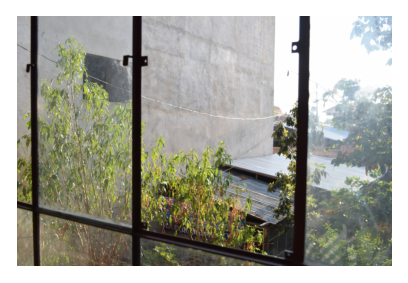
\includegraphics[width=0.293\textwidth]{img/01.luxometro.07.eps} &

\includegraphics[width=0.293\textwidth]{img/01.luxometro.08.eps} &

\includegraphics[width=0.293\textwidth]{img/01.luxometro.09.eps}
\tabularnewline \hline
\textbf{10:00} & \textbf{11:00} & \textbf{12:00} \tabularnewline
$L=(158.0\pm1)[lx], 0.63\%$ &
$L=(98.0\pm1)[lx], 1.02\%$ &
$L=(82.0\pm1)[lx], 1.22\%$ \tabularnewline

\includegraphics[width=0.293\textwidth]{img/01.luxometro.10.eps} &
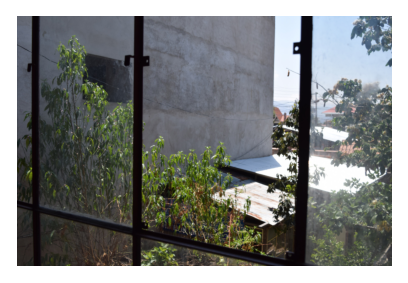
\includegraphics[width=0.293\textwidth]{img/01.luxometro.11.eps} &
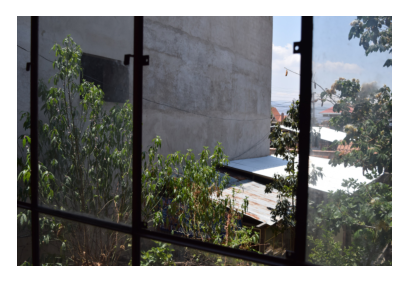
\includegraphics[width=0.293\textwidth]{img/01.luxometro.12.eps}
\tabularnewline \hline
\textbf{13:00} & \textbf{14:00} & \textbf{15:00} \tabularnewline
$L=(65.0\pm1)[lx], 1.54\%$ &
$L=(63.0\pm1)[lx], 1.59\%$ &
$L=(89.0\pm1)[lx], 1.12\%$ \tabularnewline
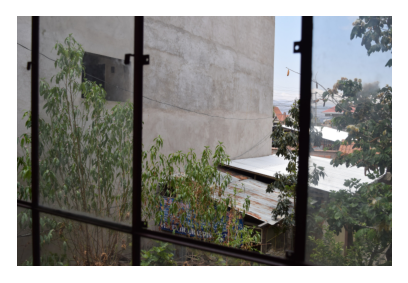
\includegraphics[width=0.293\textwidth]{img/01.luxometro.13.eps} &
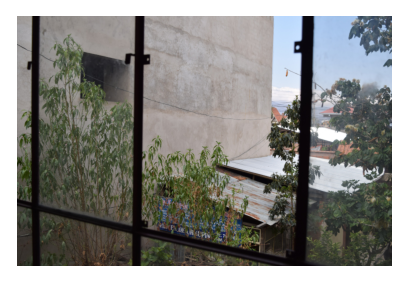
\includegraphics[width=0.293\textwidth]{img/01.luxometro.14.eps} &
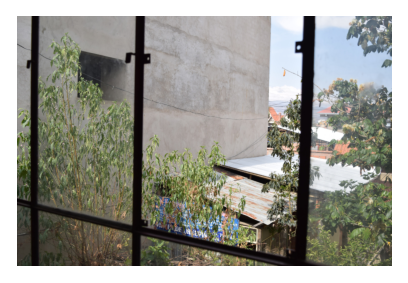
\includegraphics[width=0.293\textwidth]{img/01.luxometro.15.eps}
\tabularnewline \hline
\textbf{16:00} & \textbf{17:00} & \textbf{18:00} \tabularnewline
$L=(34.0\pm1)[lx], 2.94\%$ &
$L=(9.0\pm1)[lx], 11.11\%$ &
$L=(3.0\pm1)[lx], 33.33\%$ \tabularnewline

\includegraphics[width=0.293\textwidth]{img/01.luxometro.16.eps} &
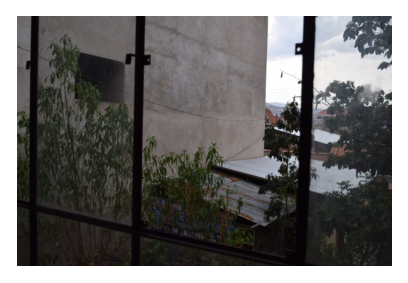
\includegraphics[width=0.293\textwidth]{img/01.luxometro.17.eps} &
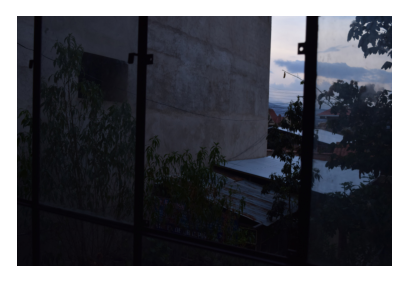
\includegraphics[width=0.293\textwidth]{img/01.luxometro.18.eps}
\tabularnewline \hline
\end{tabular}


\section{Conclusiones}
Se han obtenido medidas directas a partir de la toma de series de medidas,
y la toma de medidas unicas con instrumentos, se ha notado la importancia del
manejo de la precisión en la toma de muestras, ademas se ha visto que las
herramientas estadísticas brindan una ayuda vital a la tarea en laboratorio.

\section{Referencias bibliográficas}
\begin{itemize}
\item Fisicanet \\
https://www.fisicanet.com.ar/fisica/mediciones/ap01-mediciones-errores.php
\item Desviación típica \\
https://es.wikipedia.org/wiki/Desviación\_típica
\end{itemize}

\end{document}
